\section{Differentiated Bertrand}

Two firms $i \in \{1, 2\}$ sell imperfectly substitutable goods. They compete in Bertrand fashion by posting prices $p_i \in [0, 1]$. When they set prices $(p_1, p_2)$ the demand for firm 1’s good is $q_1(p_1, p_2) = 1 - p_1 + p_2$ and the demand for firm 2’s good is $q_2(p_2, p_1) = 1 - p_2 + p_1$. There are no costs of production, so the profit functions of the firms are
    
\[
\pi_1(p_1, p_2) = p_1(1 - p_1 + p_2)
\]
\[
\pi_2(p_2, p_1) = p_2(1 - p_2 + p_1)
\]

\begin{tcolorbox}
(a) Calculate the best-response functions $BR_1(p_2)$ and $BR_2(p_1)$ and draw them in $(p_1, p_2)$-space.
\end{tcolorbox}

For $BR_1(p_2)$:

\begin{eqnarray*}
\pi_1(p_1, p_2) &=& p_1(1 - p_1 + p_2)\\
\frac{d\pi_1}{dp_1} &=& 1 - 2p_1 + p_2 = 0
\end{eqnarray*}

From the F.O.C. we get:

\begin{eqnarray*}
p_2^* &=& 2p_1 - 1\\
p_1^* &=& \frac{1 + p_2}{2}
\end{eqnarray*}

In the same way, for $BR_2(p_1)$:

\begin{eqnarray*}
\pi_2(p_2, p_1) &=& p_2(1 - p_2 + p_1)\\
\frac{d\pi_2}{dp_2} &=& 1 - 2p_2 + p_1 = 0
\end{eqnarray*}

Therefore, from the F.O.C.:

\begin{eqnarray*}
p_1^* &=& 2p_2 - 1\\
p_2^* &=& \frac{1 + p_1}{2}
\end{eqnarray*}

\begin{myanswerbox}
    So the best response functions are:
    \begin{eqnarray*}
        p_1^* &=& \frac{1 + p_2}{2}\\
        p_2^* &=& \frac{1 + p_1}{2}
    \end{eqnarray*}
\end{myanswerbox}

\begin{figure}[htpb]
    \centering
    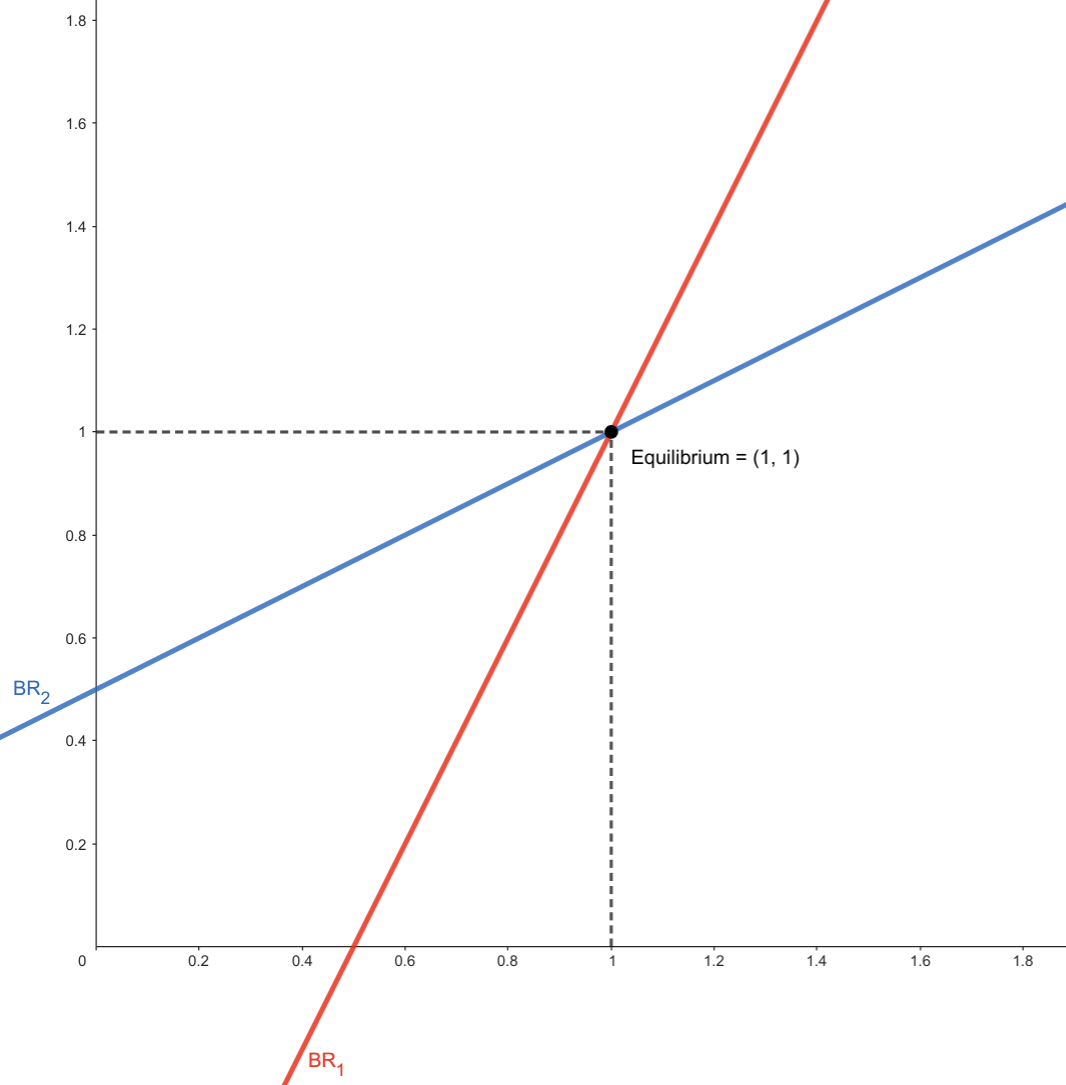
\includegraphics[scale=0.4]{plots/plot1.png}
    \caption{Best response functions}
    \label{fig:my_label}
\end{figure}

\begin{tcolorbox}
    (b) Calculate the Nash equilibrium prices $(p_1^*, p_2^*)$.
\end{tcolorbox}
    
The Nash equilibrium is the intersection of the best response functions, so:
    
\begin{eqnarray*}
p_1^* &=& \frac{1 + p_2}{2}\\
p_2^* &=& \frac{1 + p_1}{2}
\end{eqnarray*}
    
Substituting $p_1^*$ into $p_2^*$:
    
\begin{eqnarray*}
p_2^* &=& 2(2p_2 - 1) - 1\\
p_2^* &=& 4p_2 - 3\\
p_2^* &=& \frac{3}{3} = 1
\end{eqnarray*}
    
and substituting $p_2^*$ into $p_1^*$:
    
\begin{eqnarray*}
p_1^* &=& 2(1) - 1\\
p_1^* &=& 1
\end{eqnarray*}
    
\begin{myanswerbox}
    So the Nash equilibrium is $p_1^* = 1$ and $p_2^* = 1$.
\end{myanswerbox}